\documentclass[11 pt]{article} 
\usepackage[left=2cm, top=2cm, right=2cm, bottom=2.5cm, footskip=.5cm]{geometry}
\usepackage{graphicx}
\usepackage{subcaption} 
\usepackage{subfig}
\usepackage{amsmath}
\usepackage{url}
\usepackage{booktabs}
\usepackage{units}
\usepackage{enumitem}
\usepackage{listings}
\usepackage{float}
\usepackage{booktabs}
%\usepackage{hyperref}

\author{Natalia Zuniga-Garcia}
\title{Exercises 4 Better Online Learning}
\date{October 9, 2017}

\begin{document}

\maketitle


\section{Improving SGD for logistic regression}

The two techniques we learned on the last set of exercises---line search and Quasi-Newton methods---give us inspiration for how to pick the step size in stochastic gradient descent.

Let's try the following approach, called AdaGrad (adaptive gradient descent).  You'll remember that in the quasi-Newton method you implemented on the last exercises, your steps looked like this:
$$
\beta^{(t+1)} = \beta^{(t)} - \gamma^{(t)} \Omega^{(t)} \nabla l(\beta^{(t)}) \, ,
$$
where:
\begin{itemize}
	\item $\nabla l(\beta^{(t)})$ was the gradient vector, evaluated at the current estimate.
	\item $\Omega^{(t)}$ was an approximation to the inverse Hessian matrix, updated at each step according to the BFGS recursion.
	\item $\gamma^{(t)}$ was a scalar step-size parameter, chosen by line search.
\end{itemize}
This looks just like Newton's method, except that $\Omega^{(t)}$ is an approximate inverse Hessian rather than the true inverse Hessian (hence quasi-Newton).  You will have noticed that, compared with gradient-descent, the quasi-Newton method converged in many, many fewer iterations.  That's because the matrix $\Omega^{(t)}$ has the effect of re-scaling each component of the gradient vector by some amount that depends on the curvature of the objective at that point.  Low curvature means a large step size is safer along that direction; high curvature means you need to be more conservative along that direction, because you might overshoot the minimum.  Scaling by the \emph{inverse} Hessian---or in the case of quasi-Newton, an estimate of this matrix---accomplishes this rescaling.

You could certainly imagine applying a similar idea to stochastic gradient descent.  That is, you could make your updates look like this:
\begin{equation}
\label{eqn:online_quasi_newton}
\beta^{(t+1)} = \beta^{(t)} - \Omega^{(t)} g_t(\beta^{(t)}) \, ,
\end{equation}
where just as before, $g_t$ is the contribution to the gradient from the single data point processed at step $t$.  Here we've absorbed the step size into the matrix $\Omega^{(t)}$, which you should think of as exactly like the approximate inverse Hessian $\Omega^{(t)}$ that arises in quasi-Newton methods.

However, this scheme suffers from two drawbacks.  First, if we use something like the BFGS update rule to update $\Omega^t$ using the $g_t$'s at each stage, we'll end up with a super noisy Hessian.  That's because our single-data-point observations are noisy, their gradient contributions are even noisier, and their Hessian contributions are noisier still.  The following R snippet will convince you of the general principle that noise accumulates very fast as you take higher-order finite differences of something noisy.

\newpage
\begin{verbatim}
x = seq(0,4*pi, length=1000)

# Slightly noisy cosine curve
sigma = 0.025
y = cos(x) + rnorm(1000, 0, sigma)

# Function is easy to see despite the noise
plot(x, y, pch=19, col='grey')
curve(cos(x), add=TRUE, col='red', lwd=2)

# First differences are super noisy despite small sigma
plot(tail(x,-1), diff(y)/diff(x), pch=19, col='grey')
curve(-sin(x), add=TRUE, col='red', lwd=2)  # true first derivative

# Second differences? Yikes!
plot(tail(x,-2), diff(diff(y))/diff(diff(x)))
\end{verbatim}

\vspace{2mm}
\textbf{Solution}

\vspace{2mm}
Figure 1 shows the results of the previous example.

\begin{figure}[H]
	\begin{center}
		\begin{subfigure}[h]{0.35\linewidth}
			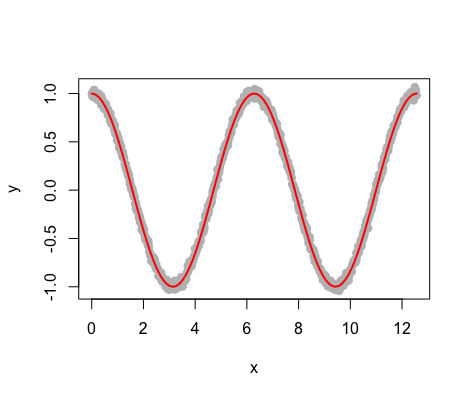
\includegraphics[width=\linewidth]{R_Code/Fig/P1F1.png}
			\caption{Function is easy to see despite the noise}
		\end{subfigure}
		\begin{subfigure}[h]{0.35\linewidth}
			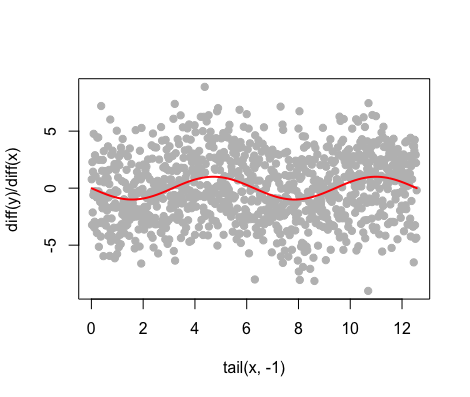
\includegraphics[width=\linewidth]{R_Code/Fig/P1F2.png}
			\caption{First differences are super noisy despite small sigma}
		\end{subfigure}
		\begin{subfigure}[h]{0.35\linewidth}
			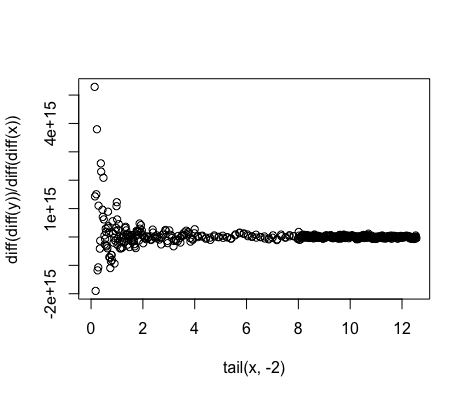
\includegraphics[width=\linewidth]{R_Code/Fig/P1F3.png}
			\caption{Second differences? Yikes!}
		\end{subfigure}
		\caption{Example of Noise Accumulating Fast}
		\label{fig:Fig1}
	\end{center}
\end{figure}


In Equation \ref{eqn:online_quasi_newton} above, na\"ively applying the BFGS update rule to calculate $\Omega$ using the noisy gradients is like trusting the second and third pictures generated by this code snippet as good approximations to the first and second derivatives.  We're effectively asking to get a reasonable approximation to the Hessian using finite differences of noisy observations.  You should be wary of this.

Equally worrying, however, is the issue of scalability.  Calculating the matrix-vector product $\Omega^{(t)} g_t(\beta^{(t)})$ requires $O(p^2)$ multiplications, where $p$ is the number of regression coefficients.\footnote{This ignores the cost of updating $\Omega$, which adds even more flops.}  This isn't a big deal if $p$ is small.  But if $p$ is large, then we've somewhat defeated the main advantage of stochastic gradient descent, which is that processing a single data is super fast: only a dot product of two length-$p$ vectors, which is linear in $p$ rather than quadratic.

The AdaGrad update rule addresses both problems.  It says: let's use a \textit{diagonal} approximation to the inverse Hessian matrix, updating the matrix at each step using $g_t$.  Because we're only estimating $p$ numbers on that diagonal (rather than $p(p+1)/2$ entries in the full inverse Hessian), there are fewer quantities to estimate, and the noise in $g_t$ hurts us less.  And if $\Omega$ is diagonal, then the cost of calculating $\Omega^{(t)} g_t(\beta^{(t)})$ scales linearly, not quadratically, in $p$.

The AdaGrad rule for tuning the SGD step size was originally proposed in a paper from 2011 by Duchi et.~al.\footnote{Duchi, John; Hazan, Elad; Singer, Yoram (2011). "Adaptive subgradient methods for online learning and stochastic optimization."  Journal of Machine Learning Research 12: 2121--59.  Duchi was a Ph.D student at the time, and the technique described in this paper more or less went straight into deployment at every major tech firm you've heard of.  They all use SGD, and the AdaGrad rule is darn useful.}  You are obviously welcome to read it, but unless you are already an expert at convex optimization and online learning, you will almost surely find it incomprehensible.  (I certainly did the first time I read it---although try revisiting it after the semester is over!)  Luckily there are many sources out there that explain the basic AdaGrad rule in plainer language.  The Wikipedia page\footnote{\url{https://en.wikipedia.org/wiki/Stochastic_gradient_descent#AdaGrad}} is just fine here.  Here are some other references:

\begin{itemize}
	
\item A nice blog post with a lot of other stuff about stochastic gradient descent: \\ \url{http://sebastianruder.com/optimizing-gradient-descent/index.html#adagrad} 
\item Another blog post with some nice pseudo-code: \\ \url{https://xcorr.net/2014/01/23/adagrad-eliminating-learning-rates-in-stochastic}  \\ \url{-gradient-descent/}
\item Some slides from a friend of mine, Emily Fox, at U.~Washington.  (These are a bit more technical.)
\url{https://courses.cs.washington.edu/courses/cse547/15sp/slides/adagrad.pdf}
\end{itemize}
And of course, Google is your friend.  Read up on AdaGrad and implement it.  How does it work for when used on one of your earlier, familiar data sets?


\newpage
\textbf{Solution}

Using the AdaGrad algorithm, we modify the Stochastic Gradient Descend (SGD) algorithm to update $\beta_j$ as follow,

$$\beta^{(k+1)}_j = \beta^{(k)}_j - \gamma_j^{(k)} \left ( \nabla l(\beta^{(k)})_j + \lambda \beta^{(k)}_j \right)$$

where, 
$$\gamma_j^{(k)} = \frac{\eta}{\sqrt{G_j}} \nabla \tilde{l}(\beta^{(k)})_j$$

 $\eta$ is the default step size, and
 $G_j$ is a diagonal matrix where each diagonal element is the sum of the squares of the gradients up to time step k. 
  
and,
\[ \lambda = \left\{ \begin{array}{lll}
- \lambda & \mbox{if $\beta_j < 0$}\\
0 & \mbox{if $\beta_j = 0$}\\
\lambda & \mbox{if $\beta_j > 0$}
\end{array} \right. \]

\newpage
\section{Putting it all together on some biggish data}

By now you've got the ice cream for your SGD sundae.  Now think about these possibilities:
\begin{itemize}
	\item Support for sparse matrices (i.e.~situations where your $X$ matrix has a lot of zeros in it).  Remember the speed-ups and reduced memory requirements that are possible by exploiting the sparsity of the $X$ matrix.\footnote{The example below probably won't run if you don't represent the data as a sparse matrix. }  A key issue that you'll have to solve is: how do I \emph{iterate efficiently} over the entries in a sparse matrix?  This is intimately related to the way your sparse matrix is stored.  It is efficient to iterate column by column, but not row by row, in a column-oriented sparse matrix.  Similarly, it is efficient to iterate row by row, but not column by column, in a column-oriented sparse matrix.
	\item Adding an $\ell^1$ regularizer, i.e.~the addition of a penalty term to the original objective that stabilizes your estimates (which will modify the gradients in a straightforward way).\footnote{Consult the course page for some reading about this idea, if it is unfamiliar.}  This corresponds to optimizing the objective
	$$
	\tilde{l}(\beta) = l(\beta) + \lambda \sum_{j=1}^p |\beta_j| \, ,
	$$
	where $\lambda$ is a scalar penalty and $l(\beta)$ is the negative log likelihood.  You'll have to modify your gradient calculation here.  Note that derivative of $|x|$ is either $\pm 1$ depending on the sign of $x$.  The exception is at zero, where the gradient is undefined.  But SGD will still work fine if you simply pretend that the derivative of $|x|$ at $x=0$ is 0.
	\item Lazy updates.  If $x_{jt}$ is zero at iteration $t$ of SGD, can you avoid have to actually touch the corresponding $\beta_j$?  This is a huge efficiency improvement if you can figure out how to do it correctly.
	\item Implementation in a compiled language (e.g.~using Rcpp and either RcppArmadillo or RcppEigen if you're working in R).
	\item Streaming data off disk in chunks, so that you don't have to load everything into memory at once.  There are several R packages appropriate for this, e.g. \verb|readr|, \verb|LaF| or \verb|stream| (there are probably others, maybe even better ones).
\end{itemize}

Aim for speed.  SGD is supposed to be fast :-)

Once you've got your code up and running (using either AdaGrad or minibatch line search), apply SGD to fit a logistic regression model to the data here\footnote{\url{http://archive.ics.uci.edu/ml/datasets/URL+Reputation}}, on detecting malicious URLs in web traffic.  It has about 2.4 million observations and 3.2 million features (so $p > n$).   Forget about random sampling here---just stream through the data one observation at a time, in the order they sit in the file.\footnote{As a benchmark, my code (which has all the ``sprinkles'' mentioned above except for the last one) takes about 13 seconds on a MacBook Pro to pass through this data set once, once it's been loaded into memory.  It is reasonably efficient, but not super optimized or anything like that.   I'll be very pleased if you can beat this!  I'll have to think of a prize here.}  As a final step, try splitting the data into training and test sets.  Fit the model on the training set, and then make predictions on the testing set.  How well does your model perform?

The course web page gives you some pointers and code for pre-processing this data.  And remember, you can probably learn a lot from your classmates on this one.

\newpage
\subsection{Optional}


Another way of thinking about the step size in SGD is using a variant on line search:
\begin{enumerate}[label=\arabic*.]
	\item At some point during the learning, select a small subsample (a ``minibatch'') of the observations as a calibration set.
	\item Try out various step sizes $\gamma$ on this subsample (using the averaged gradient from this subsample as the search direction), and pick the $\gamma$ that leads to the best fit on the calibration set.
	\item Use this step size for awhile.
\end{enumerate}
You then repeat this every so often to refresh the step size, which will end up decaying naturally over time.

Note: this way of choosing the step size based on a minibatch is \textit{almost} exactly the same as line search for regular gradient descent, treating that minibatch as the full data set.  The only difference is that the search direction vector is the \textit{average} gradient contribution for all the observations in the minibatch, rather than the sum of all gradient contributions.  These two vectors have the same direction but different length.  You need the one whose length scales like that of a single $g_t$ vector---and thus the average---to get the right step size for gradient-descent steps based on a single $g_t$.

Feel free to try this if you want, but it's not required.
	
	
	
	%\newpage
	%\bibliographystyle{ieeetr}
	%\bibliography{references}
	



	
\end{document}